\chapter{Optimal Respiratory Navigator Configuration}

\begin{center}
	\textit{Adapted from Hamlet SM, Haggerty CM, Suever JD, Wehner GJ, Andres KN, Powell DK, Zhong X, Fornwalt BK. Optimal Configuration of Respiratory Navigator Gating for the Quantification of Left Ventricular Strain Using Spiral Cine Displacement Encoding with Stimulated Echoes (DENSE) MRI. Journal of Magnetic Resonance Imaging. 2017. 45(3):796-794}
\end{center}

The purpose of this work was to determine the optimal respiratory navigator gating configuration for the quantification of left ventricular strain using spiral cine displacement encoding with stimulating echoes (DENSE) MRI.  In this chapter, we detail the different respiratory navigator configurations, their advantages and disadvantages, and the experimental protocol. This study identifies the optimal respiratory navigator configuration in adults and children compared to the "gold-standard" breath-hold acquisition.

\section{Synopsis}
	\noindent \textbf{Purpose:} To determine the optimal respiratory navigator gating configuration for the quantification of left ventricular strain using spiral cine displacement encoding with stimulated echoes (DENSE) MRI.
	
	\noindent \textbf{Methods:} Two-dimensional spiral cine DENSE was performed on a 3 Tesla MRI using two single-navigator configurations (retrospective, prospective) and a combined “dual-navigator” configuration in 10 healthy adults and 20 healthy children. The adults also underwent breathhold DENSE as a reference standard for comparisons. Peak left ventricular strains, signal-to-noise ratio (SNR), and navigator efficiency were compared. Subjects also underwent dual-navigator gating with and without visual feedback to determine the effect on navigator efficiency.
	
	\noindent \textbf{Results:} There were no differences in circumferential, radial, and longitudinal strains between navigator-gated and breath- hold DENSE (P~=~0.09---0.95) (as confidence intervals, retrospective: [-1.0\%--1.1\%], [-7.4\%--2.0\%], [-1.0\%$–$1.2\%]; prospective: [-0.6\%--2.7\%], [-2.8\%--8.3\%], [-0.3\%--2.9\%]; dual: [-1.6\%--0.5\%], [-8.3\%--3.2\%], [-0.8\%--1.9\%], respectively). The dual configuration maintained SNR compared with breathhold acquisitions (16 versus 18, P~=~0.06). SNR for the prospective configuration was lower than for the dual navigator in adults (P~=~0.004) and children (P~$<$~0.001). Navigator efficiency was higher (P~$<$~0.001) for both retrospective (54\%) and prospective (56\%) configurations compared with the dual configuration (35\%). Visual feedback improved the dual configuration navigator efficiency to 55\% (P~$<$~0.001).
	
	\noindent \textbf{Conclusion:} When quantifying left ventricular strains using spiral cine DENSE MRI, a dual navigator configuration results in the highest SNR in adults and children. In adults, a retrospective configuration has good navigator efficiency without a substantial drop in SNR. Prospective gating should be avoided because it has the lowest SNR. Visual feedback represents an effective option to maintain navigator efficiency while using a dual navigator configuration.
	
	\noindent \textbf{Keywords:} Respiratory Navigator, Breath-holds, DENSE, Strain, Signal-to-Noise Ratio, Navigator Efficiency\\
	
	\newpage

\section{Introduction}
	Magnetic resonance (MR) can be used to non-invasively assess cardiac function. Displacement encoding with stimulated echoes (DENSE) is an advanced cardiac MR imaging technique that directly measures tissue displacements and can be used to quantify cardiac mechanics, such as myocardial strains and torsion \cite{Aletras1999,Aletras1999a}. When combined with clinical risk factors, these measures of cardiac mechanics have been shown to be better predictors of mortality than traditional measures of cardiac function, such as ejection fraction \cite{Stanton2009}.
	 
	Compensation for respiratory motion is an important consideration for all cardiac MR techniques, particularly quantitative imaging sequences like spiral cine DENSE. DENSE acquisitions are generally performed using end-expiratory breath-holds ($\sim$15–-20 seconds in duration) \cite{Kim2004,Zhong2006,Ernande2012,Zhong2010a,Aletras2005,Spottiswoode2007,Young2012c}; however, this approach is constrained by the patient's ability to breath-hold, which is limited in young subjects and many stages of advanced heart disease. Furthermore, short acquisitions preclude the ability to capture more robust data, such as three-dimensional (3D) DENSE \cite{Zhong2010a,Kar2014,Auger2012}, or high resolution imaging \cite{Wehner2014}.
	
	As with many other cardiac MR sequences, a respiratory navigator has been used to overcome this time limitation by allowing the subject to breathe freely but restricting data acquisition based on the position of the diaphragm within a prescribed 'acceptance' window \cite{Zhong2010a}. However, unlike some other MR sequences, the navigator echo in the DENSE sequence cannot occur at the beginning of the cardiac cycle, since this would lead to interference with displacement encoding. Instead, the navigator echo must occur at the end of the cardiac cycle, immediately after data acquisition. This creates several options for how the navigator can then be used to either accept or reject the acquired DENSE data (Figure~\ref{fig:navigator_configurations}). For example, a single echo can be used retrospectively or prospectively to define acceptance of DENSE data from the current or preceding cardiac cycle, respectively. Alternatively, a dual-navigator configuration can be used, which requires an echo from the current and preceding cardiac cycle to define acceptance of DENSE data (Figure~\ref{fig:navigator_configurations}). Each configuration has distinct advantages and disadvantages. For example, compared to the single navigator configurations, the dual-navigator configuration has more rigorous criteria for correctly accepting data (Figure~\ref{fig:navigator_advantages_disadvantages}). However, these strict criteria likely lead to worse navigator efficiency compared to the single navigator configurations (Figure~\ref{fig:navigator_advantages_disadvantages}).
	
	Previous studies using navigator-gated DENSE have reported using a prospective single navigator configuration \cite{Zhong2010a,Auger2012}. However, there has been no formal comparison of the available navigator configurations. Moreover, the accuracy of derived cardiac mechanics and overall image quality for these navigator configurations compared with breath-hold acquisitions as a reference standard are largely unknown. The purpose of this study was to determine the optimal configuration of respiratory navigator gating for the quantification of left ventricular strain using spiral cine DENSE MRI.

\begin{figure} 
	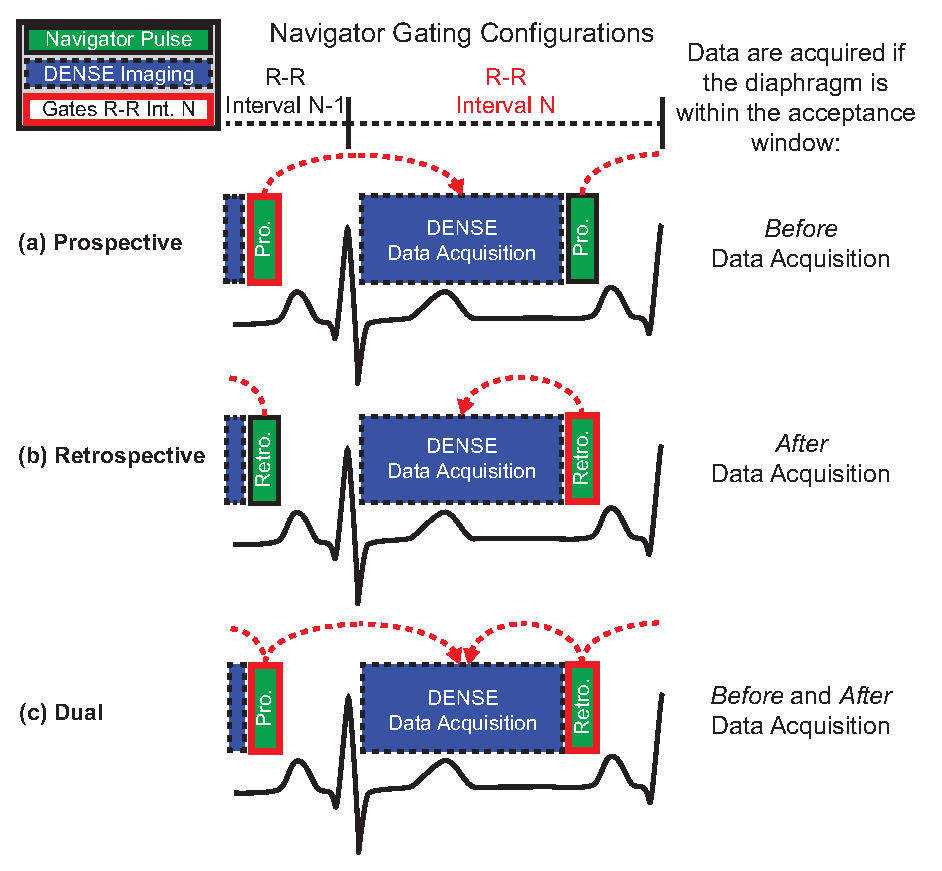
\includegraphics{figures/navpaper/Fig1}
	\caption[Different navigator gating configurations used to acquire DENSE image data]{\textbf{Different navigator gating configurations used to acquire DENSE image data.} The single navigator configurations: (\textbf{A}) prospective and (\textbf{B}) retrospective; and the (\textbf{C}) dual navigator configuration. The red outlines and arrows indicate which navigator pulse(s) is/are gating the DENSE data acquisition.}
	\label{fig:navigator_configurations}
\end{figure}

\begin{figure} 
	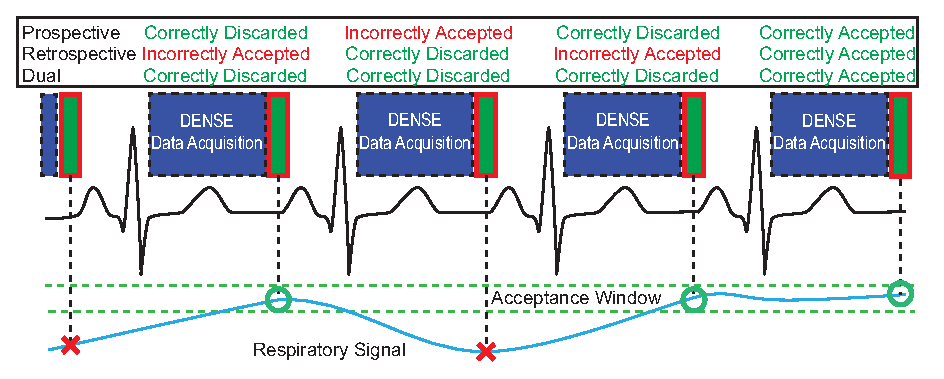
\includegraphics{figures/navpaper/Fig2}
	\caption[Theoretical example to demonstrate the disadvantages of single- and dual-navigator gating configurations]{\textbf{Theoretical example to demonstrate the disadvantages of single- and dual-navigator gating configurations.} The red colored text identifies the incorrectly accepted DENSE data from single-navigator gating configurations (i.e. the diaphragm is not within the acceptance window for the entirety of DENSE data acquisition, but the data are still accepted). The number of “Accepted/Discarded” data in the example above illustrate how a dual navigator gating configuration will discard more data compared to single navigator gating configurations (retrospective and prospective) and lead to lower navigator efficiency. The red 'x' or green 'o' represents the detected diaphragm location being outside or inside the acceptance window, respectively.}
	\label{fig:navigator_advantages_disadvantages}
\end{figure}

\section{Methods}

\subsection{Subjects}
	Ten healthy adults and 20 healthy children with no known history of cardiovascular disease or chronic illnesses and a normal 12-lead electrocardiogram were prospectively enrolled. The protocol was approved by the local Institutional Review Board and all subjects provided informed consent (or assent/parental consent, as appropriate).

\subsection{Image Acquisition}
	Image acquisition was performed on a 3T Siemens Tim Trio (Siemens Healthcare, Erlangen, Germany) with a 6-element chest coil and a 24-element spine coil. 2D spiral cine DENSE \cite{Zhong2010a,Wehner2015} in mid-ventricular short-axis and four-chamber long-axis orientations were separately acquired using breath-holds and retrospective, prospective, and dual navigator gating. Due to the lengthy breath-hold duration ($\sim$20 seconds), breath-hold acquisitions were not performed in children. The order of the navigator gating configurations was randomized. Prospective ECG gating was used and the number of cardiac phases was selected to allow 100-150 ms at the end of the cardiac cycle for heart rate variability. Acquisition parameters for all scans were: spiral type: uniform density, interleaves = 6, interleaves per beat = 2, FOV = 360x360 mm$^2$, pixel spacing = 2.8x2.8 mm$^2$, slice thickness = 8 mm, TE = 1.1 ms, TR = 17 ms, variable flip angle = 20$^{\circ}$ \cite{Wehner2015,Stuber1999}, displacement encoding = 0.06 cyc/mm \cite{Wehner2015a}, through-plane dephasing = 0.08 cyc/mm \cite{Zhong2006} CSPAMM echo suppression \cite{Kim2004}, and view sharing. The temporal resolution was 34 ms, however sliding window view sharing yielded a 17 ms temporal resolution between reconstructed cardiac frames. Based on the DENSE parameters, acquisition duration for each orientation was 20 heartbeats.
	
	The respiratory navigator was placed over the dome of the liver. Subjects were asked to breathe comfortably and a scout navigator was used to track the diaphragm. The navigator acceptance window was placed so that the maximum acceptance window position was located 1-2 millimeters above the subject's maximum expiration position. A navigator acceptance window of $\pm$3 mm (total range of 7 mm) was used for all navigator gated scans. Navigator efficiency was measured as the number of cardiac cycles from which data were acquired and accepted over the total number of cardiac cycles required to complete a scan.

\subsection{Navigator Feedback}
	Because the dual-navigator configuration was expected to decrease navigator efficiency, we developed and tested a feedback system, which allowed the subject to view their diaphragm position in real-time during image acquisition. The goal was to compensate for reduced navigator efficiency in order to preserve the clinical feasibility of DENSE imaging using a dual-navigator configuration.
	
	The feedback system consisted of an angled mirror placed above the patient's head so that an image of the diaphragm location was viewable on a screen located at the back of the scanner bore. The image of the diaphragm location (respiratory navigator display) was projected from the scanner console's video feed onto the screen with an MRI-compatible projector. After all other scans were completed, subjects used this feedback system, with the dual-navigator gating configuration, to acquire the same short-axis and long-axis images.
	
	This feedback system was also used prior to the breath-hold scan to ensure a consistent end-expiratory diaphragm location between the navigator-gated acquisitions and the breath-hold acquisitions. With instruction, the subject exhaled and breath-held in the acceptance window, at which point the navigated scan was halted and the breath-hold acquisition was immediately performed. Breath-hold acquisitions were always performed after the navigator-gated acquisitions that did not involve navigator feedback in order to minimize the potential effect of navigator feedback on respiratory patterns.

\subsection{DENSE Post-Processing}
	All DENSE images were analyzed using custom, open-source MATLAB (The Mathworks Inc, Natick, MA) software, \textit{DENSEanalysis} \cite{Gilliam2016a}. For each set of DENSE images, endocardial and epicardial boundaries were drawn on the magnitude image from an end-diastolic and end-systolic frame. A simplified analysis technique was used to reconstruct the motion field \cite{Suever2014}. The displacement-encoded phase images were unwrapped using a path-following algorithm with manual selection of seed points. The resulting Lagrangian displacements underwent spatial smoothing and temporal fitting as previously described \cite{Spottiswoode2007}.
	
	Segmental two-dimensional Lagrangian strains were computed over the cardiac cycle for 6 segments in the short-axis images (radial and circumferential strain) and from the long-axis images (longitudinal strain). Cardiac segments were defined using the American Heart Association 17-segment model. Average peak strains were computed by averaging the strain curves of all the myocardial segments together and finding the peak of this average strain curve. When computing peak longitudinal strain, pixels within 10\% of left ventricular longitudinal length from the most basal and apical regions were excluded in order to exclude the increased noise which is typically observed in the strain curves in those regions. Thickening was defined by convention as positive strain, whereas shortening was defined as negative.

\subsection{Analysis}
	Mean modified coefficient of variation (CoV) \cite{Wehner2015a,Haggerty2013,Wehner2015} was used to measure agreement in strain between different navigator configurations and breath-holds. The calculation of the CoV is shown below where $N$ is the number of subjects and $x_1$ and $x_2$ are the strain measurements.

\begin{equation}
	\label{eq:cov}
	CoV=\frac{\Sigma_{i=1}^N[St.Dev(x_1[i],x_2[i])]/N}{|\Sigma_{i=1}^N[(x_1[i]+x_2[i])/2]/N|}
\end{equation}

	Consistent with previous studies reporting CoVs \cite{Haggerty2013,Swoboda2014,Moody2015,Kowallick2014,Kowallick2016}, results less than or equal to 20\% were considered acceptable.
	
	To compare image quality, signal-to-noise ratio (SNR) was computed using the DENSE magnitude images at end-systole. SNR was quantified from the average myocardial signal and the standard deviation of the noise within an area free from tissue or imaging artifacts \cite{Wehner2015a,Wehner2015,Sigfridsson2011}. Because the MR signal has a Rician distribution, corrections were applied in order to calculate the true SNR \cite{Gudbjartsson1995}. The measured standard deviation, $\sigma_M$, was used to compute the true standard deviation, $\sigma$, by

\begin{equation}
	\sigma = \sqrt{\frac{2}{4-\pi}}*\sigma_M \approx 1.526*\sigma_M
\end{equation}

	The measured myocardial signal, $M$, was used to compute the true myocardial signal, $S$, by

\begin{equation}
	S= \sqrt{M^2-\sigma^2}
\end{equation}

	SNR was defined as the ratio of the true myocardial signal ($S$) to the true standard deviation ($\sigma$).

\subsection{Comparison of Acquisition Configurations}
	We compared peak global and segmental strains (circumferential, radial, and longitudinal) and SNR of the end-systolic DENSE magnitude images between each acquisition technique (breath-hold and navigator gating) in adults. Bland-Altman analyses \cite{Bland1986}, CoV \cite{Haggerty2013}, and 95\% confidence intervals (CI) were used to measure agreement in strain between the separate navigator configurations and breath-holds. A paired Student's t-test was used to compare strains between navigator configurations and breath-holds. We also compared SNR and navigator efficiency between all navigator configurations (dual, retrospective, and prospective) in adults and children using a one-way repeated measures ANOVA with post-hoc analyses and Bonferroni correction. All data are presented as mean $\pm$ one standard deviation. Significance was defined as p $<$ 0.05.

\section{Results}
	Ten healthy adults (Age: 23 $\pm$ 3 years, 40\% female) and 20 healthy children (Age: 13 $\pm$ 3 years, 45\% female) were enrolled in the study. DENSE data were successfully acquired in all subjects except for one child who could not complete the study protocol due to an erratic respiratory pattern.

\subsection{Average Peak Strains}
	Average peak left ventricular strains are shown in Table~\ref{table:navigator_strains}. There were no significant mean differences in circumferential, radial, and longitudinal strain between the dual, retrospective, and prospective navigator configurations and breath-holds in adults (Figure~\ref{fig:nav_strain_bland_altman}). Compared to breath-holds, all navigator configurations had a CoV of less than 20\% for circumferential, radial, and longitudinal strain in adults (Figure~\ref{fig:nav_strain_bland_altman}). The differences in strain are listed as confidence intervals in Table~\ref{table:nav_CI_strains}. Peak segmental left ventricular strains are shown in Table~\ref{table:navigator_segmental_strains} in Appendix A). There were no significant differences in segmental strain between the navigator configurations and breath-holds except for radial strain from the prospective configuration (p = 0.002, Table~\ref{table:nav_CI_seg_strains}). Compared to breath-holds, all navigator configurations had CoVs of less than 20\% except for radial segmental strain (19-28\%) (Table~\ref{table:nav_CI_seg_strains}).

%Table 4.1
\begin{table}
	\centering
	\caption[Average strains for different acquisition techniques]{\textbf{Average strains for different acquisition techniques.}}
	\label{table:navigator_strains}
	\begin{tabular}{c  c  c}
		\toprule
		\multicolumn{1}{c}{}       			 & \multicolumn{2}{c}{\textbf{Mean $\pm$ Std. Dev.}} \\ 
		\multicolumn{1}{c}{}				 & \multicolumn{1}{c}{\textbf{Adults}} 			& \multicolumn{1}{c}{\textbf{Children}} \\ \midrule
		\multicolumn{1}{l}{\textbf{Circumferential Strain (\%)}}                       		& \multicolumn{2}{c}{} \\
		\multicolumn{1}{r}{Breath-hold}      & \multicolumn{1}{c}{-17 $\pm$ 2}              & \multicolumn{1}{c}{--}          			\\
		\multicolumn{1}{r}{Retrospective}    & \multicolumn{1}{c}{-18 $\pm$ 2}              & \multicolumn{1}{c}{-19 $\pm$ 2}           \\
		\multicolumn{1}{r}{Prospective}      & \multicolumn{1}{c}{-17 $\pm$ 3}              & \multicolumn{1}{c}{-18 $\pm$ 2}           \\
		\multicolumn{1}{r}{Dual}    		 & \multicolumn{1}{c}{-18 $\pm$ 3}              & \multicolumn{1}{c}{-20 $\pm$ 2}           \\
		\multicolumn{1}{l}{\textbf{Radial Strain (\%)}}                       				& \multicolumn{2}{c}{} \\
		\multicolumn{1}{r}{Breath-hold}      & \multicolumn{1}{c}{30 $\pm$ 10}              & \multicolumn{1}{c}{--}          			\\
		\multicolumn{1}{r}{Retrospective}    & \multicolumn{1}{c}{26 $\pm$ 9}               & \multicolumn{1}{c}{30 $\pm$ 9}           \\
		\multicolumn{1}{r}{Prospective}      & \multicolumn{1}{c}{31 $\pm$ 7}               & \multicolumn{1}{c}{26 $\pm$ 12}           \\
		\multicolumn{1}{r}{Dual}		     & \multicolumn{1}{c}{27 $\pm$ 9}               & \multicolumn{1}{c}{27 $\pm$ 12}           \\
		\multicolumn{1}{l}{\textbf{Longitudinal Strain (\%)}}                       		& \multicolumn{2}{c}{} \\
		\multicolumn{1}{r}{Breath-hold}      & \multicolumn{1}{c}{-14 $\pm$ 2}              & \multicolumn{1}{c}{--}          			\\
		\multicolumn{1}{r}{Retrospective}    & \multicolumn{1}{c}{-14 $\pm$ 2}              & \multicolumn{1}{c}{-14 $\pm$ 2}           \\
		\multicolumn{1}{r}{Prospective}      & \multicolumn{1}{c}{-13 $\pm$ 2}              & \multicolumn{1}{c}{-14 $\pm$ 2}           \\
		\multicolumn{1}{r}{Dual}		     & \multicolumn{1}{c}{-14 $\pm$ 2}              & \multicolumn{1}{c}{-14 $\pm$ 2}           \\
		\bottomrule                                                 
	\end{tabular}
\end{table}

% Figure 4.3
\begin{figure}
	\centering % center figure
	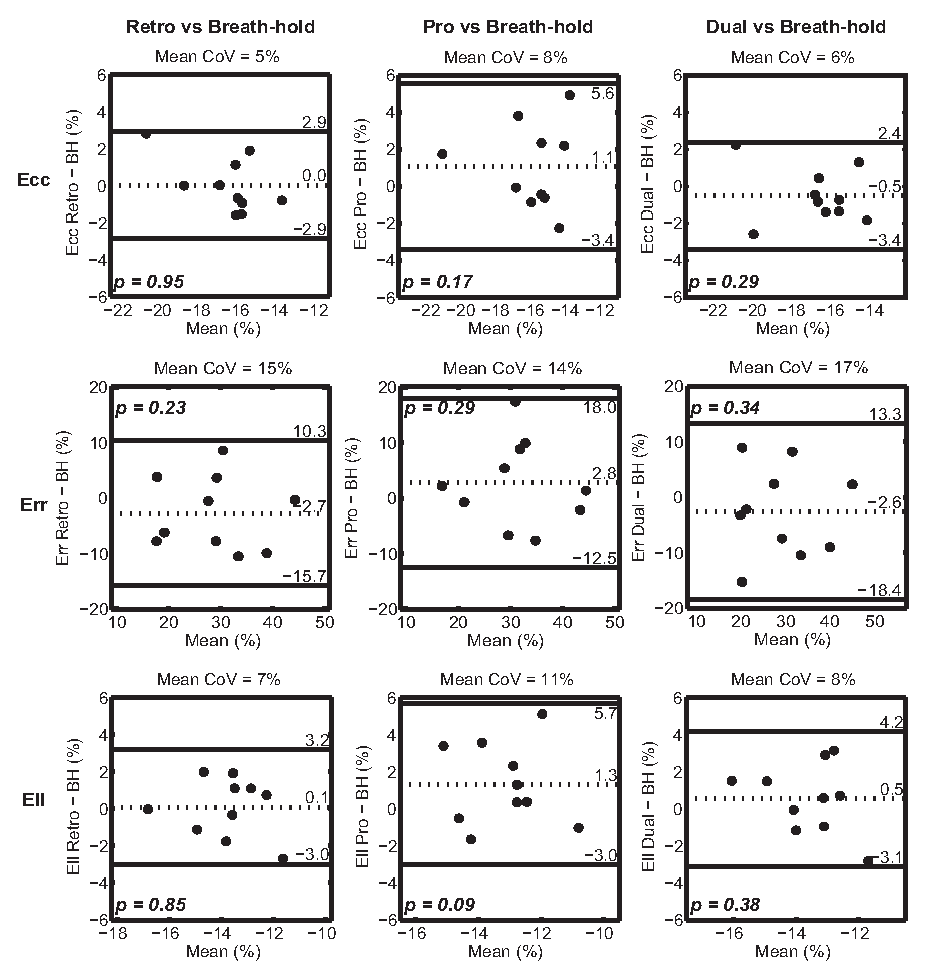
\includegraphics{figures/navpaper/Fig3}
	\caption[Bland-Altman plots of average peak circumferential (Ecc), radial (Err), and longitudinal (Ell) strains for retrospective, prospective, and dual navigator gating vs breath-hold]{\textbf{Bland-Altman plots of average peak circumferential (Ecc), radial (Err), and longitudinal (Ell) strains for retrospective, prospective, and dual navigator gating vs breath-hold.}}
	\label{fig:nav_strain_bland_altman}
\end{figure}

%Table 4.2
	\begin{table}
	\centering
	\caption[CI Results for Differences in Strain Between Navigator Gating and Breathhold DENSE]{\textbf{CI Results for Differences in Strain Between Navigator Gating and Breathhold DENSE.}}
	\label{table:nav_CI_strains}
	\begin{tabular}{c c c}
		\toprule
		\multicolumn{1}{c}{}&\multicolumn{1}{c}{\textbf{95\% LoA}} & \multicolumn{1}{c}{\textbf{p-value}}\\ \midrule
		\multicolumn{1}{l}{\textbf{Circumferential Strain (\%)}}   & \multicolumn{2}{c}{}     \\
		\multicolumn{1}{r}{Retrospective--Breath-hold}  & \multicolumn{1}{c}{[-1.0--1.1]}  & \multicolumn{1}{c}{0.95} \\
		\multicolumn{1}{r}{Prospective--Breath-hold}    & \multicolumn{1}{c}{[-0.6--2.7]}  & \multicolumn{1}{c}{0.17} \\
		\multicolumn{1}{r}{Dual--Breath-hold}           & \multicolumn{1}{c}{[-1.6-–0.5]}  & \multicolumn{1}{c}{0.29} \\
		\multicolumn{1}{l}{\textbf{Radial Strain (\%)}}            & \multicolumn{2}{c}{}     \\
		\multicolumn{1}{r}{Retrospective--Breath-hold}  & \multicolumn{1}{c}{[-7.4--2.0]}  & \multicolumn{1}{c}{0.23} \\
		\multicolumn{1}{r}{Prospective--Breath-hold}    & \multicolumn{1}{c}{[-2.8--8.3]}  & \multicolumn{1}{c}{0.29} \\
		\multicolumn{1}{r}{Dual--Breath-hold}           & \multicolumn{1}{c}{[-8.3–-3.2]}  & \multicolumn{1}{c}{0.34} \\
		\multicolumn{1}{l}{\textbf{Longitudinal Strain (\%)}}      & \multicolumn{2}{c}{}     \\
		\multicolumn{1}{r}{Retrospective--Breath-hold}  & \multicolumn{1}{c}{[-1.0–-2.0]}   & \multicolumn{1}{c}{0.85} \\
		\multicolumn{1}{r}{Prospective--Breath-hold}    & \multicolumn{1}{c}{[-0.3–-2.9]}   & \multicolumn{1}{c}{0.09} \\
		\multicolumn{1}{r}{Dual--Breath-hold}           & \multicolumn{1}{c}{[-0.8--1.9]}   & \multicolumn{1}{c}{0.38} \\
		\bottomrule                                 
	\end{tabular}
\end{table}



\subsection{Signal-to-Noise Ratio}
	In adults, single navigator configurations had a 17-28\% reduction in SNR compared to breath-hold DENSE (Table~\ref{table:navigator_snr}). There was no difference in SNR between the dual navigator configuration and breath-hold DENSE (p = 0.06). Among navigator configurations, dual and retrospective navigator configurations were comparable and both had better SNR (23\% and 15\%, respectively) compared to the prospective configuration (p = 0.02, p = 0.004, respectively).
	
	In children, SNR also differed based on navigator gating configuration (Table~\ref{table:navigator_snr}). The dual navigator configuration had the highest SNR compared to the retrospective (23\% higher, p $<$ 0.001) and prospective (35\% higher, p $<$ 0.001) configurations. There was no difference in SNR between the retrospective and prospective navigator configurations (p = 0.15).

%Table 4.5
\begin{table}
	\centering
	\caption[Signal-to-noise ratios for different navigator gating configurations in adults and children]{\textbf{Signal-to-noise ratios for different navigator gating configurations in adults and children.}}
	\label{table:navigator_snr}
	\begin{tabular}{c c c c c}
		\toprule
		\multicolumn{1}{c}{} & \multicolumn{1}{c}{\textbf{Adults}} & \multicolumn{1}{c}{\textbf{p-value}} & \multicolumn{1}{c}{\textbf{Children}} & \multicolumn{1}{c}{\textbf{p-value}} \\ \midrule
		\multicolumn{1}{r}{Breath-hold}      & \multicolumn{1}{c}{18 $\pm$ 8} & \multirow{4}{*}{$<$ 0.001} & \multicolumn{1}{c}{--} & \multirow{4}{*}{$<$ 0.001}     \\
		\multicolumn{1}{r}{Retrospective}    & \multicolumn{1}{c}{15 $\pm$ 6*$\dagger$} & & \multicolumn{1}{c}{22 $\pm$ 6$\ddagger$} &                 \\
		\multicolumn{1}{r}{Prospective}      & \multicolumn{1}{c}{13 $\pm$ 5*} & & \multicolumn{1}{c}{20 $\pm$ 8$\ddagger$} &                 \\
		\multicolumn{1}{r}{Dual}    		 & \multicolumn{1}{c}{16 $\pm$ 7} & & \multicolumn{1}{c}{27 $\pm$ 9} &                 \\
		\bottomrule
		\multicolumn{5}{l}{\footnotesize* p $<$ 0.05 vs. breath-hold; $\dagger$ p $<$ 0.05 vs. prospective; $\ddagger$ p $<$ 0.05 vs. dual} \\
	\end{tabular}
\end{table}

\subsection{Navigator Efficiency}
	For adults and children combined, there were significant differences in navigator efficiency between navigator configurations (p $<$ 0.001, Table~\ref{table:navigator_navefficiency}). The retrospective and prospective navigator configurations had higher navigator efficiencies than the dual navigator configuration by an average of 54\% (p $<$ 0.001) and 60\% (p $<$ 0.001), respectively. Using visual feedback with the dual navigator configuration improved navigator efficiency by 57\% (p $<$ 0.001) compared to the dual configuration without feedback and resulted in comparable efficiency to the single navigator configurations. The scan times mirrored the navigator efficiency results. For example, scan times for adults were, on average, 64, 37, 37, and 25 seconds for the dual, retrospective, prospective configurations, and the dual navigator configuration with feedback, respectively.

%Table 4.6
\begin{table}
	\centering
	\caption[Navigator efficiencies for different navigator gating configurations in adults and children]{\textbf{Navigator efficiencies for different navigator gating configurations in adults and children.}}
	\label{table:navigator_navefficiency}
	\begin{tabular}{c c c c c}
		\toprule
		\multicolumn{1}{c}{} & \multicolumn{1}{c}{\textbf{Pooled}} & \multicolumn{1}{c}{\textbf{p-value}} & \multicolumn{1}{c}{\textbf{Adults}} & \multicolumn{1}{c}{\textbf{Children}} \\ \midrule
		\multicolumn{1}{r}{Retrospective}   & \multicolumn{1}{c}{54 $\pm$ 15*} & \multirow{4}{*}{$<$ 0.001} & \multicolumn{1}{c}{48 $\pm$ 15*} & \multicolumn{1}{c}{57 $\pm$ 16*}     \\
		\multicolumn{1}{r}{Prospective}    	& \multicolumn{1}{c}{56 $\pm$ 15*} & & \multicolumn{1}{c}{52 $\pm$ 17*} &  \multicolumn{1}{c}{58 $\pm$ 14*}                \\
		\multicolumn{1}{r}{Dual}      		& \multicolumn{1}{c}{35 $\pm$ 13}  & & \multicolumn{1}{c}{31 $\pm$ 16} &   \multicolumn{1}{c}{37 $\pm$ 11}               \\
		\multicolumn{1}{r}{Dual Feedback}   & \multicolumn{1}{c}{55 $\pm$ 16*} & & \multicolumn{1}{c}{67 $\pm$ 11*} &   \multicolumn{1}{c}{48 $\pm$ 15*}               \\
		\bottomrule
		\multicolumn{5}{l}{\footnotesize* p $<$ 0.05 vs. dual (without feedback)} \\
	\end{tabular}
\end{table}

\section{Discussion}
	The use of respiratory navigated acquisitions for spiral cine DENSE extends the potential utility of the technique by removing restrictions on patient breath-holding abilities and allowing for high resolution \cite{Wehner2014} and/or three dimensional  \cite{Zhong2010a,Kar2014} data collection. While previous studies have used a respiratory navigator with DENSE, the optimal configuration for gating and how it might differ among subjects has been largely unexplored. This study addressed these knowledge gaps by showing that: 1) left ventricular peak strains were not different between breath-held and navigator-gated DENSE acquisitions; 2) SNR was reduced with single navigator configurations, but not the dual configuration, compared to breath-held acquisitions; 3) the SNR benefit of the dual navigator configuration was offset by reduced navigator efficiency compared to single navigator configurations, but visual navigator feedback maintained clinically acceptable efficiencies for the dual navigator acquisition. The following paragraphs explore each of these findings in greater detail.
	
	There were no significant mean differences and good paired agreement of all peak strains between retrospective, prospective, and dual navigator configurations and breath-holds in adults. This finding agrees with the prior work by Zhong et al., which compared segmental strains from navigator-gated 3D DENSE to breath-hold 2D DENSE \cite{Zhong2010a} and similarly reported clinically acceptable agreement. Our study extends this work by demonstrating that the agreement exists not only for prospective navigator-gating used by Zhong et al., but for retrospective and dual navigator-gating configurations as well. Demonstrating this agreement of strain values—a primary endpoint for most DENSE acquisitions—has pragmatic value by ensuring that data from acquisitions with differing respiratory compensation can be readily compared.
	
	Our results demonstrate that using a single navigator configuration resulted in significantly lower SNR compared to breath-hold DENSE acquisitions. While this result was only demonstrated in adults because of the prohibitively long breath-hold duration in children, it is reasonable to assume that a similar trend holds in children as well. Among the navigator configurations, the dual configurations provided the best SNR as it was superior to prospective navigator gating in both adults and children, had better SNR than retrospective gating in children, and resulted in comparable SNR to breath-hold DENSE.
	
	Differences in SNR among the different acquisitions are likely attributable to heart rate and respiratory variability. The breath-hold acquisitions had the shortest acquisition time, with presumably less physiologic variability. Also, the dual navigator configuration had the most stringent acceptance criteria, which likely minimized the effects of respiratory variability during acquisition compared to the other configurations. This reasoning is supported by previous studies, which have reported associations between consistent diaphragm position during navigator-gated acquisitions and improved SNR \cite{Feuerlein2009,Jhooti2011}. In both adults and children, the prospective navigator configuration had the lowest SNR of all navigator configurations. The observed difference in SNR between the single navigator configurations was perhaps unexpected given the theoretical similarities in their design and function. However, these differences are similarly attributable to the effects of variability: for the retrospective navigator, the interval between the R wave and the navigator echo is fixed, whereas heart rate changes during the scan will affect the interval between the navigator echo and the succeeding R wave in prospective gating, increasing the likelihood of respiratory variability during that interval. Based on these findings, the use of prospective navigator gating for DENSE should be avoided.
	
	Notably, a previous study compared SNR of a 2D steady-state free precession sequence between dual navigator-gated and breath-hold acquisitions and found that end-systolic myocardial SNR for breath-hold acquisitions was 23\% lower than the dual navigator configuration in adults \cite{Peters2008}. This finding contrasts with our data in which the dual navigator configuration was statistically comparable to breath-hold. However, the previous study had substantially different imaging parameters between their dual navigator-gated acquisition and the breath-hold acquisition, which likely accounted for the observed SNR differences \cite{Peters2008}.
	
	Although the purpose of this study was to determine the optimal navigator gating strategy, it is worth noting that SNR was higher for children than it was for adults. The difference in SNR between adults and children is likely related to the smaller body habitus of children, which results in a shorter distance between the MRI coils and the heart. Moreover, adults likely have more adipose tissue, which could also lead to lower SNR. Ultimately, these SNR differences may lead to differences in inter-test reproducibility between adults and children.
	
	As expected, single navigator gating configurations resulted in better navigator efficiency compared to dual navigator gating, due to the additional acceptance criteria constraints of the dual navigator. Simply put, more data are discarded with dual navigator gating, leading to prolonged scan time. Previous studies using a single-navigator configuration with the same size acceptance window ($\pm$3 mm) reported navigator gating efficiencies ranging from 20 to 48\% \cite{Zhong2010a,Feuerlein2009,Abd-Elmoniem2011}. Compared to these studies, we observed slightly better single-navigator efficiencies of 48 to 52\% in adults and 57 to 58\% in children. The dual navigator efficiency was comparable to results from previous studies \cite{Peters2008}.
	
	To potentially offset this reduced efficiency, we evaluated the effect of providing the subject with visual feedback of the diaphragm position, which has been shown to considerably improve navigator efficiency compared to traditional free-breathing acquisitions \cite{Feuerlein2009}. We found that using visual feedback during dual navigator gated acquisitions improved navigator efficiency compared to the dual configuration without feedback and resulted in comparable efficiency to the single navigator configurations. The improvement with feedback was not uniform across adults and children (i.e., the improvement in kids was not as substantial), perhaps reflecting the superior ability of the adults to hold their breath within the acceptance window. Alternatively, the difference may be indicative of the non-intuitive nature of the respiratory navigator display and the differential abilities of adults and kids to quickly learn and use it. Efforts are ongoing to instead transform this image to a more kid-friendly video game design to improve usability \cite{Hamlet2016a}.
	
	The increased scan time associated with the dual navigator configuration presents an obvious trade-off with improved SNR for its utility in a clinical setting where time is a critical consideration. In adults, given the minimal difference in SNR between the dual and retrospective navigator configurations, the substantial drop in efficiency with the dual navigator may not be justified. In children, however, the SNR benefit with dual navigator gating is more substantial and warrants consideration to ensure high quality data. Hence the demonstrated improvement in navigator efficiency by providing the subject with visual feedback is an important finding because it provides one option for compromise: achieving improved SNR while approximately maintaining scan time compared to other navigator configurations.
	
	This study was performed using 2D DENSE. However, given the similarity in the fundamental sequence designs of 2D and 3D DENSE, the results are applicable to 3D DENSE acquisitions as well. In fact, given the longer time generally required for 3D data acquisition, respiratory compensation/navigation is essential, so these results are highly relevant. Specifically, our navigator efficiency findings agree with reported efficiencies from a previous study using 3D DENSE \cite{Zhong2010a}. Also, while absolute magnitudes of SNR may differ with more data acquired, there is no reason to suspect that the relative differences in SNR would change between different navigator gating strategies when applying these results to 3D DENSE.
	
	A limitation of this study is the potentially limited power for detecting small strain differences between navigator configurations and breath-hold DENSE. However, our study had 80\% power to detect a difference of 1.5\% between the retrospective navigator configuration and breath-holds. This 1.5\% difference is smaller than the typical inter-test limits of agreement of circumferential strain \cite{Wehner2015a}. Moreover, even if the strains from the prospective navigator configuration, which had the worst agreement, are in fact different from the breath-hold technique, the conclusions of the study would not change as the prospective navigator configuration was separately found to be sub-optimal based on SNR.
	
	Another limitation was the lack of breath-hold data for the pediatric subjects. The DENSE acquisition required 20 heartbeats. The required breath-hold time was further extended by the use of a navigator-gated pre-scan to ensure that breath-holds were performed at the same diaphragm position as the navigator-gated scans. This duration was viewed to be prohibitively long for pediatric subjects, and so no breath-hold DENSE data were acquired in these cases. The equivalence of DENSE-derived strains between breath-hold and navigator sequences was demonstrated in adults. Since children did not undergo breath-hold DENSE, we must caution future studies regarding these strain results as they apply to children. However, since the relative SNR and navigator efficiency results from navigator gating were similar to those in adults, we would expect potential differences to be small. Furthermore, the primary objective of the study was to identify optimal navigator configurations for DENSE, so the lack of breath-hold data in children is a minor limitation.
	
	A third limitation of this study is the lack of assessment of clinical patients. Cardiac patients, who routinely undergo MR imaging and who may have limited ability to hold their breath, may not be able to perform the lengthy breath-hold scan and may not achieve as high navigator efficiency when performing a dual navigator scan with feedback. However, since this population is more likely to undergo DENSE MR imaging than this study's volunteer subjects, it would be beneficial to determine whether the results remain the same. For example, it may be important to use dual navigator gating, even at the expense of navigator efficiency, to achieve higher SNR, since SNR is commonly lower in the clinical patient population compared to healthy volunteers.
	
	In conclusion, for spiral cine DENSE acquisitions, respiratory navigator gating and breath-hold acquisitions yield comparable values of left ventricular peak strains. However, differences in signal-to-noise ratios and navigator efficiencies were observed among the different navigator gating configurations, which warrant consideration in clinical and research protocol design. In adult subjects, the dual navigator configuration produced the best SNR, although only slightly better than the single retrospective navigator, which produced acceptable SNR and therefore may be used to maintain good efficiency. For children, the benefit of a dual navigator configuration for improved SNR was even more apparent, but resulted in a considerable drop in scan efficiency. The prospective navigator resulted in the poorest SNR and should be avoided. The use of visual navigator feedback represents an effective option to maintain navigator efficiency while using the dual navigator in children (and adults).